\chapter{Feuerbälle, Bezugssysteme und Vierervektoren}

Wir beginnen mit einer Frage, die nach der Diskussion hochenergetischer Kollisionen offen geblieben ist. Bei der Kollision zweier schwerer Atomkerne entsteht ein heftig veränderliches Objekt, kein ruhiges astronomisches Schwarzes Loch. Was kann es also bedeuten, die Kollision mithilfe eines Horizonts zu beschreiben? Die Antwort führt über ein fünfdimensionales Bild stark gekoppelter Materie und einige praktische Fragen zu Beschleunigern schließlich zurück zur Geometrie der speziellen Relativitätstheorie. Am Ende sind Geschwindigkeit und Impuls zu Vierervektoren geworden, und die Energie steht neben den drei Impulskomponenten.

\section{Ein Feuerball in einer fünften Dimension}

\begin{classroomqa}
\audiencequestion{Das bei der Kollision entstehende Objekt ist instabil und verändert seine Form. Wie kann man ein so komplexes Objekt als Schwarzes Loch bezeichnen?}
\lecturerresponse{Stellen wir uns eine fünfte räumliche Richtung zwischen einem Boden und einer Decke vor. Die Gravitation in dieser Richtung zieht Anregungen zum Boden hin. Bei der Kollision wird dort ein heißer Energieklumpen abgelagert; er breitet sich aus und verändert seine Form, kann aber dennoch einen Horizont, eine Temperatur und eine Entropie besitzen.}
\end{classroomqa}

Stellen wir uns Teilchen oder, anschaulicher, kleine Strings vor, die sich in dieser fünfdimensionalen Welt bewegen. Anregungen, die zum Boden fallen, erscheinen in vier Dimensionen als Hadronen: Protonen, Neutronen, Mesonen und andere ausgedehnte zusammengesetzte Objekte. Anregungen nahe der Decke erscheinen elementarer. Die vertikale Position kodiert somit die Skala auf geometrische Weise: Der Boden steht für den hadronischen Bereich großer Abstände, die Decke für Freiheitsgrade bei kleinen Abständen.

Wenn zwei Hadronen kollidieren, stoßen zwei Objekte nahe dem Boden zusammen und erzeugen eine große Energiefreisetzung. Das Ergebnis ist kein starrer Körper, sondern ein heißer Klumpen mit Horizont, eine Art Pfütze im fünfdimensionalen Gravitationsfeld. Es ist weder ein astronomisches Schwarzes Loch im gewöhnlichen vierdimensionalen Raum noch ein Schwarzes Loch auf der Planck-Skala, das an der Decke sitzt. Es ist die gravitative Beschreibung des stark wechselwirkenden Feuerballs nahe dem Boden.

Bei hohen Energien werden die einlaufenden Atomkerne lorentzkontrahiert und zu dünnen Pfannkuchen. Sie kollidieren, deponieren ihre Energie in einem kleinen Gebiet und erzeugen ein Fluid, das sich zum Gleichgewicht hin ausbreitet. Seine geringe Viskosität war eine der überraschenden Eigenschaften des Quark--Gluon-Plasmas. In der fünfdimensionalen Beschreibung entspricht dieselbe Entwicklung der Relaxation eines verzerrten Horizonts.

\begin{figure}[H]
\centering
\includegraphics[width=0.82\textwidth]{lecture_05_figure_01.png}
\caption{Das Bild der fünften Dimension mit Boden und Decke. Der zentrale Klumpen mit Horizont breitet sich nach der Kollision entlang des Bodens aus.}
\lectureframe{00:04:22}
\end{figure}

Ein Horizont bleibt nicht ewig bestehen. Hawking-Strahlung trägt Energie davon, und in der vierdimensionalen Beschreibung ist diese Strahlung der Schauer gewöhnlicher Hadronen, die aus der Kollision hervorgehen. Die Tausenden Spuren in einem Detektorereignis sind in dieser Sprache die Teilchen, die aus dem dualen Schwarzen Loch herausgesiedet sind.

\subsection{Ist die zusätzliche Dimension real?}

\begin{classroomqa}
\audiencequestion{Ist die fünfte Dimension eine räumliche Dimension, und erstreckt sich die zwischen Boden und Decke gezeichnete Linie buchstäblich in diese Richtung?}
\lecturerresponse{Ja. Sie ist raumartig, und die in dieser fünfdimensionalen Geometrie gezeichnete Fläche ist ein Horizont. Ob man die zusätzliche Richtung als ``real'' bezeichnet oder sie als gleichwertige mathematische Beschreibung auffasst, ist eine tiefer gehende Frage.}
\end{classroomqa}

Die nützliche Aussage lautet nicht, dass die Gravitation die Quantenchromodynamik ersetzt. Vielmehr können zwei Sprachen dieselbe Physik beschreiben. In der vierdimensionalen Sprache gibt es einen heißen Feuerball aus Quarks und Gluonen, aber kein gewöhnliches Gravitationsfeld. In der fünfdimensionalen Sprache gibt es Gravitation und einen Horizont. Wenn die Korrespondenz stimmt, müssen eine korrekte QCD-Rechnung und die duale Gravitationsrechnung überall dort übereinstimmen, wo sich beide durchführen lassen.

\begin{classroomqa}
\audiencequestion{QCD kennt weder Gravitation noch Horizonte. Fügt das Bild des Schwarzen Lochs neue Physik hinzu, oder beschreibt es den Feuerball lediglich anders?}
\lecturerresponse{In vier Dimensionen ist es ein Plasma aus Quarks und Gluonen; in seiner fünfdimensionalen Ausprägung besitzt es eine gravitative Beschreibung mit einem Horizont. Der Vorteil liegt in der Berechnung. Stark gekoppelte QCD ist äußerst schwierig, während sich manche Eigenschaften des Horizonts---insbesondere die Viskosität---vergleichsweise leicht berechnen lassen.}
\end{classroomqa}

Die Frage, ob es sich um eine ``reale Dimension'' oder eine ``mathematische Analogie'' handelt, muss nicht geklärt werden, bevor die Beschreibung nützlich sein kann. Eine Struktur erhält eine physikalische Deutung, wenn sie die übrigen Variablen zu einem einfacheren und kohärenteren Satz von Gesetzen zusammenführt. Dennoch sollte man die Aussage nicht übertreiben: Anwendungen der Eich-Gravitation-Dualität auf das beobachtete Quark--Gluon-Plasma sind Modelle stark gekoppelter Dynamik und kein Beweis dafür, dass es für die QCD der realen Welt ein bekanntes exaktes gravitationelles Dual gibt.\editorialnote{Diese Einschränkung macht den heutigen Stand der QCD-Anwendung ausdrücklich deutlich; sie ändert nichts am hier entwickelten fünfdimensionalen Mechanismus.}

\section{Warum Beschleuniger kollidierende Strahlen verwenden}

Nun werden die Fragen praktisch. Warum verwendet man zwei bewegte Strahlen statt eines einzelnen Strahls und eines ruhenden Ziels? Warum sind kreisförmige Beschleuniger so groß? Warum geht man mit Elektronen und Protonen unterschiedlich um? All diese Fragen betreffen relativistische Energie.

\begin{classroomqa}
\audiencequestion{Warum lässt man zwei Strahlen miteinander kollidieren, statt einen energiereichen Strahl auf ein ruhendes Ziel zu richten?}
\lecturerresponse{Für die Erzeugung neuer Teilchen ist die im Schwerpunktsystem verfügbare Energie maßgeblich. Zwei gleich starke, entgegengesetzt gerichtete relativistische Strahlen haben keinen Gesamtimpuls, sodass im Wesentlichen ihre gesamte Energie für die Kollision zur Verfügung steht. Bei einem ruhenden Ziel bleibt ein großer Teil der einfallenden Energie als Bewegung des Schwerpunkts gebunden.}
\end{classroomqa}

Für zwei ultrarelativistische Teilchen mit entgegengesetzten Impulsen vom Betrag \(p\) lautet die Abschätzung auf Vorlesungsniveau in Einheiten mit \(c=1\)
\begin{equation}
E_{\mathrm{cm}}^{\mathrm{collider}}\simeq 2p.
\end{equation}
Die entsprechende Abschätzung für ein ruhendes Ziel wächst nur mit der Quadratwurzel des Strahlimpulses:
\begin{equation}
E_{\mathrm{cm}}^{\mathrm{fixed}}\sim \sqrt{mp}.
\end{equation}
Entscheidend ist die Skalierung, nicht der weggelassene Zahlenfaktor: Eine Verdopplung der Strahlenergie verdoppelt die Kollisionsenergie des Beschleunigers, erhöht die Schwerpunktsenergie beim ruhenden Ziel aber nur um einen Faktor gleich der Quadratwurzel.

Die invariante Rechnung macht den Vergleich präzise. Sind \(P_1\) und \(P_2\) die einlaufenden Viererimpulse, gilt
\begin{equation}
s=(P_1+P_2)^2,
\qquad E_{\mathrm{cm}}=\sqrt{s}.
\end{equation}
Für zwei gleichenergetische, entgegengesetzt laufende Strahlen mit Energie \(E\) heben sich die räumlichen Impulse auf, sodass \(\sqrt{s}=2E\) gilt. Für ein Projektil der Energie \(E\gg m\), das auf ein ruhendes Ziel gleicher Masse trifft, gilt
\begin{equation}
s=2m^2+2mE,
\qquad
\sqrt{s}\simeq \sqrt{2mE}
\qquad (c=1).
\end{equation}
Diese kurze Herleitung mit Invarianten liefert den Faktor, der in der mündlichen Abschätzung unterdrückt wurde.\editorialnote{Die Herleitung ist hier aufgenommen, damit sich das Skalierungsargument der Vorlesung nachvollziehen lässt.}

\begin{classroomqa}
\audiencequestion{Gibt es einen grundlegenden Grund dafür, dass ein kreisförmiger Beschleuniger so groß sein muss? Könnte derselbe Strahl nicht einfach öfter durch eine kleinere Maschine kreisen?}
\lecturerresponse{Felder und Materialien setzen Grenzen. Ein Teilchen gewinnt pro Meter nur eine begrenzte Energie, daher braucht eine Maschine für höhere Energien eine größere wirksame Beschleunigungsstrecke. Ein enger Kreis erfordert zudem eine größere Querbeschleunigung, und eine beschleunigte Ladung strahlt. Ist der Ring zu klein, strahlt der Strahl Energie genauso schnell ab, wie die Maschine sie zuführt.}
\end{classroomqa}

Die Beziehung für die Ablenkung lautet näherungsweise
\begin{equation}
p=qBR,
\end{equation}
Bei festem Magnetfeld \(B\) erfordert ein größerer Impuls \(p\) also einen größeren Radius \(R\). Die Hochfrequenzkavitäten verrichten die Arbeit, die die Strahlenergie erhöht; die Magnete lenken den Strahl ab und fokussieren ihn. Die grundsätzliche Aussage bleibt die an der Tafel erläuterte: Die Feldstärke und die Strahlungsverluste hindern uns daran, einen beliebig energiereichen Beschleuniger in einen kleinen Ring zu packen.

Bei einer Kreisbewegung tritt auch bei konstanter Geschwindigkeit eine Beschleunigung auf, denn die Geschwindigkeit ändert ihre Richtung. Eine beschleunigte Ladung sendet Synchrotronstrahlung aus. Ein Linearbeschleuniger vermeidet den kontinuierlichen Ablenkungsverlust, auch wenn die kurzen Beschleunigungsstöße selbst nicht buchstäblich strahlungsfrei sind. Kreisförmige Maschinen nehmen die Kosten der Ablenkung in Kauf und verwenden dafür bei jedem Umlauf dieselbe Anlage erneut.

\begin{classroomqa}
\audiencequestion{Warum wurden Elektronen mit dem Linearbeschleuniger am SLAC in Verbindung gebracht, während kreisförmige Hochenergie-Collider Protonen oder andere Hadronen verwenden?}
\lecturerresponse{Elektronen sind viel leichter. Bei gleicher hoher Energie ist ihr Lorentzfaktor deutlich größer, und bei kreisförmiger Beschleunigung strahlen sie viel stärker. Schwerere Protonen können wiederholt im Kreis laufen und bei jedem Umlauf Energie gewinnen, bevor Synchrotronverluste untragbar werden.}
\end{classroomqa}

Bei gleicher Energie und gleichem Ringradius hängt die Strahlungsleistung sehr stark von der Teilchenmasse ab:
\begin{equation}
P_{\mathrm{sync}}\propto \frac{E^4}{m^4R^2}.
\end{equation}
Darum ist der Unterschied zwischen Elektronen und Protonen--deutlich ausgeprägter, als die Formulierung ``das leichtere Teilchen bewegt sich schneller'' vermuten lässt: Beide Strahlen können bereits sehr nahe an \(c\) liegen, aber ihre Lorentzfaktoren und Strahlungsverluste unterscheiden sich stark.\editorialnote{Die Ablenkungsbeziehung und die Skalierung der Synchrotronstrahlung präzisieren das qualitative Argument der Vorlesung zu Beschleunigern; an der Tafel wurden sie nicht hergeleitet.}

\begin{classroomqa}
\audiencequestion{Warum beschleunigt man Hadronen nicht ebenfalls geradlinig?}
\lecturerresponse{Das ist möglich. Die Schwierigkeit liegt in der Länge. In einem Ring durchläuft dasselbe Teilchen die Beschleunigungsstrukturen viele Male; eine gleichwertige lineare Hadronenmaschine müsste enorm lang sein. Ein sinnvoller Kompromiss ist ein großer Ring, groß genug, damit die Protonenstrahlung erträglich bleibt.}
\end{classroomqa}

Diese Fragen zu Beschleunigern machen genau deutlich, weshalb die Newtonsche Mechanik nicht ausreicht. Wir wenden uns nun wieder der speziellen Relativitätstheorie zu und entwickeln die Sprache, mit der sich solche Vergleiche systematisch führen lassen.

\section{Die Garage und die Limousine}

Betrachten wir eine etwa zwölf Fuß lange Garage und eine etwa zwanzig Fuß lange Stretchlimousine. Der Fahrer beschleunigt, bis die Limousine lorentzkontrahiert ist, und hofft, dass sie hineinpasst. Im Bezugssystem der Garage ist die bewegte Limousine kürzer, sodass es möglich erscheint. Im Bezugssystem der Limousine dagegen ist die bewegte Garage kürzer, sodass es unmöglich erscheint. Kann sich die gesamte Limousine in der Garage befinden?

Öffnen wir beide Tore, damit uns eine mögliche Kollision mit einer Wand nicht ablenkt. Die Aussage, dass sich die Limousine in der Garage befindet, bedeutet, dass sich ihr Vorder- und Hinterende \emph{gleichzeitig} in der Garage befinden. Dieses letzte Wort enthält das ganze Rätsel.

Zeichnen wir ein Raum-Zeit-Diagramm mit \(t\) als vertikaler und \(x\) als horizontaler Achse. Lichtstrahlen bilden in Einheiten mit \(c=1\) einen Lichtkegel mit Öffnungswinkel \(45^\circ\). Die Garage ruht, daher sind die Weltlinien ihrer beiden Tore vertikal. Vorder- und Hinterende der Limousine beschreiben zwei parallele, schräge Weltlinien. Die \(t'\)-Achse des bewegten Bezugssystems ist zum Lichtkegel hin geneigt, und seine Simultanitätslinien verlaufen parallel zur geneigten \(x'\)-Achse.

\begin{figure}[H]
\centering
\includegraphics[width=0.82\textwidth]{lecture_05_figure_02.png}
\caption{Das vollständige Raum-Zeit-Diagramm für Garage und Limousine. Vertikale Linien begrenzen die Garage; schräge Linien zeichnen die beiden Enden der Limousine nach. Horizontale und geneigte Schnitte stellen die unterschiedlichen Simultanitätsebenen der beiden Bezugssysteme dar.--}
\lectureframe{00:31:05}
\end{figure}

Im Bezugssystem der Garage kann eine horizontale Linie beide Weltlinien der Limousine zwischen den beiden Weltlinien der Garagentore schneiden. Zu diesem Zeitpunkt im Garagenbezugssystem ist das Heck bereits eingefahren, während die Front noch nicht wieder hinausgefahren ist. Die kontrahierte Limousine befindet sich vollständig in der Garage.

Im Bezugssystem der Limousine liegen die relevanten gleichzeitigen Ereignisse auf einer geneigten Linie. Zeichnen wir eine solche Linie durch das Ereignis, bei dem das Heck einfährt. Sie trifft die Weltlinie der Front, nachdem diese bereits am weiter entfernten Tor vorbeigefahren ist. Nach der für sie maßgeblichen Gleichzeitigkeit befindet sich die Limousine also niemals vollständig in der Garage. Beide Aussagen sind wahr, weil sie jeweils unterschiedliche Ereignispaare vergleichen.

\begin{classroomqa}
\audiencequestion{Bilden die beiden grünen Weltlinien und das horizontale Segment zwischen ihnen ein Parallelogramm? Ist dieses schwarze Segment die Länge des Fahrzeugs?}
\lecturerresponse{Das horizontale Segment ist die lorentzkontrahierte Länge, denn seine Endpunkte sind im Bezugssystem der Garage gleichzeitig. Die Ruhelänge erhält man mit Endpunkten, die im Bezugssystem der Limousine gleichzeitig sind, auf einer Linie parallel zu \(x'\). Die beiden Messungen verwenden unterschiedliche Schnitte durch dasselbe Weltlinienpaar.}
\end{classroomqa}

Ist \(L_0\) die Ruhelänge, dann hat der horizontale Schnitt im Bezugssystem der Garage die Länge
\begin{equation}
L=\frac{L_0}{\gamma},
\qquad
\gamma=\frac{1}{\sqrt{1-v^2/c^2}}.
\end{equation}
Die Formel allein löst das Paradoxon nicht. Das leistet das Diagramm, weil es zeigt, welche Ereignisse miteinander verglichen wurden. Scheint ein Relativitätsrätsel zwei unvereinbare Antworten zu liefern, sollte man nach einer unausgesprochenen Verwendung des Wortes ``gleichzeitig'' suchen.

\section{Vier Koordinaten und zwei Indexstellungen}

Um von Rätseln zu Bewegungsgesetzen überzugehen, brauchen wir eine Notation, die die Geometrie berücksichtigt. Wir fassen die Koordinaten wie folgt zusammen:
\begin{equation}
(X^1,X^2,X^3,X^0)=(x,y,z,t),
\qquad X^\mu=(x,y,z,t),
\end{equation}
Dabei durchläuft \(\mu\) die Werte \(1,2,3,0\). Auf der Seite steht die Zeit an letzter Stelle, obwohl ihr Index \(0\) ist; damit folgen wir der Konvention an der Tafel.

\begin{classroomqa}
\audiencequestion{Setzen wir \(c=1\)? Sollte bei Rückkehr zu den üblichen Einheiten die Zeitkoordinate \(ct\) lauten?}
\lecturerresponse{Ja. Bei der Entwicklung der Geometrie setzen wir \(c=1\) und fügen die Faktoren \(c\) wieder ein, wenn Dimensionen oder der nichtrelativistische Grenzfall eine Rolle spielen. In den üblichen Längeneinheiten lautet die Zeitkoordinate \(ct\).}
\end{classroomqa}

Derselbe Vektor lässt sich auch mit einem unteren Index schreiben. Bei der hier verwendeten Vorzeichenkonvention gilt
\begin{equation}
X_\mu=(-x,-y,-z,t).
\end{equation}
Beim Senken eines Index wechseln also die Vorzeichen der drei räumlichen Komponenten, während die Zeitkomponente unverändert bleibt. Zum Beispiel:
\begin{equation}
X^\mu=(3,2,4,10)
\quad\Longrightarrow\quad
X_\mu=(-3,-2,-4,10).
\end{equation}
Das sind keine zwei Raum-Zeit-Punkte, sondern zwei Komponentendarstellungen desselben geometrischen Objekts.

\begin{classroomqa}
\audiencequestion{Welche Komponenten sind kovariant und welche kontravariant, und sind die Bezeichnungen als Hoch- oder Tiefstellungen gemeint?}
\lecturerresponse{Komponenten mit oberen Indizes sind kontravariant, solche mit unteren Indizes kovariant. Als Eselsbrücke aus dem Hörsaal gilt: ``co steht unten, kontra steht oben.'' Physiker sagen oft einfach „oben“ und „unten“.}
\end{classroomqa}

Die Notation bewährt sich bei der invarianten Kontraktion
\begin{equation}
X_\mu X^\mu=t^2-x^2-y^2-z^2.
\label{eq:l5-interval}
\end{equation}
In Differentialform lautet sie
\begin{equation}
d\tau^2=dt^2-dx^2-dy^2-dz^2
\qquad (c=1).
\label{eq:l5-proper-time}
\end{equation}
Bei zeitartiger Bewegung ist \(d\tau\) die Zeit, die eine Uhr entlang der Weltlinie misst.

Tritt derselbe Index einmal oben und einmal unten auf, wird über ihn summiert. Einsteins Summenkonvention verkürzt
\begin{equation}
\sum_{\mu}X_\mu X^\mu
\end{equation}
zu dem kürzeren Ausdruck in Gl.~\eqref{eq:l5-interval}. Das ist nicht bloß typografische Vereinfachung. So müssen die wechselnden Vorzeichen der Minkowski-Geometrie nicht in jeder Gleichung von Hand neu ausgeschrieben werden.

\begin{classroomqa}
\audiencequestion{Ist \(\tau\) das übliche Symbol für die Eigenzeit?}
\lecturerresponse{Ja. Manchmal wird auch das Symbol \(s\) verwendet, aber \(\tau\) ist eine übliche Wahl für die Eigenzeit.}
\end{classroomqa}

\section{Drehungen als einfache Symmetrie}

Ein Lorentz-Boost mischt Raum und Zeit. Bevor wir diese Matrix untersuchen, betrachten wir die vertrautere Operation, die räumlichen Achsen zu drehen. Zeigt die Relativbewegung in eine beliebige Richtung, können wir die Achsen so drehen, dass diese Richtung zur neuen \(x\)-Achse wird, und anschließend den bekannten Boost anwenden. Drehungen sind also Teil der Konstruktion und kein bloßer Umweg.

Bei einer Drehung um die \(z\)-Achse mit dem Winkel \(\theta\) gilt
\begin{align}
x'&=x\cos\theta+y\sin\theta,\nonumber\\
y'&=-x\sin\theta+y\cos\theta,\label{eq:l5-rotation}\\
z'&=z.\nonumber
\end{align}
Für \(\theta=0\) ergeben diese Gleichungen wieder \(x'=x\) und \(y'=y\); für \(\theta=\pi/2\) vertauschen sie die Achsen mit den erwarteten Vorzeichen.

Die Transformation erhält den euklidischen Abstand. Setzen wir
\(c_\theta=\cos\theta\) und \(s_\theta=\sin\theta\), so gilt
\begin{align}
x'^2+y'^2
&=(xc_\theta+ys_\theta)^2+(-xs_\theta+yc_\theta)^2\nonumber\\
&=x^2(c_\theta^2+s_\theta^2)
  +y^2(s_\theta^2+c_\theta^2)\nonumber\\
&\quad+2xyc_\theta s_\theta-2xyc_\theta s_\theta\nonumber\\
&=x^2+y^2.
\end{align}
Die gemischten Terme heben sich auf und \(c_\theta^2+s_\theta^2=1\). Da \(z'=z\) gilt, ist die gesamte Länge \(x^2+y^2+z^2\) invariant.

Dieselben Gleichungen lassen sich zu einer einzigen Matrixgleichung zusammenfassen:
\begin{equation}
\begin{pmatrix}x'\\y'\\z'\end{pmatrix}
=
\underbrace{\begin{pmatrix}
\cos\theta&\sin\theta&0\\
-\sin\theta&\cos\theta&0\\
0&0&1
\end{pmatrix}}_{M}
\begin{pmatrix}x\\y\\z\end{pmatrix}.
\label{eq:l5-rotation-matrix}
\end{equation}
In Indexnotation lautet sie
\begin{equation}
x'^i=M^i{}_{j}x^j,
\qquad i,j=1,2,3.
\end{equation}

\begin{figure}[H]
\centering
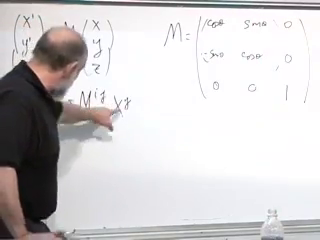
\includegraphics[width=0.82\textwidth]{lecture_05_figure_03.png}
\caption{Die räumliche Drehung, dargestellt sowohl als Matrixgleichung als auch in Indexnotation.}
\lectureframe{01:00:40}
\end{figure}

\section{Lorentz-Matrizen und zusammengesetzte Geschwindigkeiten}

Für eine Bewegung entlang \(x\) lautet die Lorentz-Transformation in Einheiten mit \(c=1\)
\begin{align}
x'&=\gamma_v(x-vt), & y'&=y,\nonumber\\
z'&=z, & t'&=\gamma_v(t-vx),
\end{align}
Dabei ist
\begin{equation}
\gamma_v=\frac{1}{\sqrt{1-v^2}}.
\end{equation}
Bei der Komponentenreihenfolge \((x,y,z,t)\) ergibt sich
\begin{equation}
\begin{pmatrix}x'\\y'\\z'\\t'\end{pmatrix}
=
\begin{pmatrix}
\gamma_v&0&0&-\gamma_vv\\
0&1&0&0\\
0&0&1&0\\
-\gamma_vv&0&0&\gamma_v
\end{pmatrix}
\begin{pmatrix}x\\y\\z\\t\end{pmatrix}.
\label{eq:l5-lorentz-matrix}
\end{equation}

\begin{figure}[H]
\centering
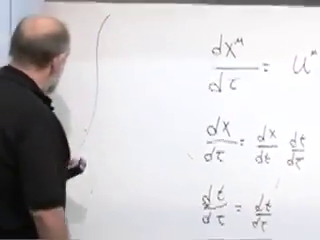
\includegraphics[width=0.82\textwidth]{lecture_05_figure_04.png}
\caption{Die \(4\times4\)-Lorentz-Matrix. Nur die Komponenten \(x\) und \(t\) werden gemischt; \(y\) und \(z\) bleiben unverändert.}
\lectureframe{01:04:40}
\end{figure}

Die Matrixmultiplikation beantwortet nun eine physikalische Frage. Nehmen wir an, ein Beobachter bewegt sich relativ zu uns mit der Geschwindigkeit \(v\), und ein dritter Beobachter bewegt sich relativ zu ihm mit der Geschwindigkeit \(u\), jeweils entlang derselben Achse. Die Newtonsche Kinematik ergäbe \(w=u+v\); damit könnten sich zwei Geschwindigkeiten von jeweils \(3c/4\) zu \(3c/2\) addieren. Die Relativitätstheorie muss eine andere Regel liefern.

Der aktive Teil des Boosts ist die \(2\times2\)-Matrix
\begin{equation}
B(v)=\gamma_v
\begin{pmatrix}1&-v\\-v&1\end{pmatrix}.
\end{equation}
Durch die Zusammensetzung der beiden Boosts ergibt sich
\begin{align}
B(u)B(v)
&=\gamma_u\gamma_v
\begin{pmatrix}1&-u\\-u&1\end{pmatrix}
\begin{pmatrix}1&-v\\-v&1\end{pmatrix}\nonumber\\
&=\gamma_u\gamma_v
\begin{pmatrix}
1+uv&-(u+v)\\
-(u+v)&1+uv
\end{pmatrix}.
\label{eq:l5-composed-boost}
\end{align}
Das Verhältnis eines Nebendiagonaleintrags zu einem Diagonaleintrag bestimmt die Geschwindigkeit des resultierenden Boosts:
\begin{equation}
w=\frac{u+v}{1+uv}
\qquad(c=1).
\end{equation}
Mit wiederhergestellten Einheiten lautet die Beziehung
\begin{equation}
w=\frac{u+v}{1+uv/c^2}.
\label{eq:l5-velocity-addition}
\end{equation}

\begin{figure}[H]
\centering
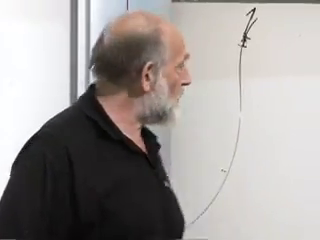
\includegraphics[width=0.82\textwidth]{lecture_05_figure_05.png}
\caption{Die Matrix des zusammengesetzten Boosts und die Geschwindigkeit \(w=(u+v)/(1+uv)\) in natürlichen Einheiten.}
\lectureframe{01:15:35}
\end{figure}

Sind \(u\) und \(v\) jeweils nahe an \(c\), nähert sich der Zähler \(2c\), während sich der Nenner \(2\) nähert. Somit nähert sich \(w\) dem Wert \(c\) und nicht \(2c\). Allgemeiner bildet Gl.~\eqref{eq:l5-velocity-addition} unterluminale Eingangsgeschwindigkeiten auf ein unterluminales Ergebnis ab. Die Matrixmultiplikation berücksichtigt die Geschwindigkeitsgrenze automatisch.

\section{Vierervektoren und das Versagen der gewöhnlichen Geschwindigkeit}

Ein Vierervektor ist ein beliebiges Objekt, dessen vier Komponenten sich bei Drehungen und Lorentz-Boosts genauso transformieren wie die Raum-Zeit-Koordinaten. Ist \(V^\mu\) ein Vierervektor, so gilt bei unserer Vorzeichenkonvention
\begin{equation}
V_\mu=(-V^1,-V^2,-V^3,V^0),
\end{equation}
und für seine invariante Norm
\begin{equation}
V_\mu V^\mu=(V^0)^2-(V^1)^2-(V^2)^2-(V^3)^2.
\end{equation}
Auch für zwei Vierervektoren \(V^\mu\) und \(W^\mu\) ist die Kontraktion
\begin{equation}
W_\mu V^\mu
=W^0V^0-W^1V^1-W^2V^2-W^3V^3
\end{equation}
invariant. Die Komponenten ändern sich beim Übergang zwischen Bezugssystemen; die Kontraktion bleibt unverändert.

Die gewöhnliche Geschwindigkeit hat nur drei Komponenten:
\begin{equation}
\mathbf v=\left(\frac{dx}{dt},\frac{dy}{dt},\frac{dz}{dt}\right).
\end{equation}
Das Anhängen von \(dt/dt=1\) macht sie noch nicht zu einem brauchbaren Vierervektor. Die vierte Komponente wäre trivial, und das so entstehende Objekt würde sich unter Lorentz-Transformationen nicht linear transformieren. Die Koordinatenzeit \(t\) ändert sich von einem Bezugssystem zum anderen; die Ableitung nach \(t\) zerstört daher das gewünschte Transformationsgesetz.

Die Eigenzeit schafft Abhilfe. Entlang einer Weltlinie definieren wir
\begin{equation}
u^\mu=\frac{dX^\mu}{d\tau}.
\label{eq:l5-four-velocity}
\end{equation}
Das Differential \(dX^\mu\) ist ein Vierervektor und \(d\tau\) invariant, also ist auch ihr Quotient ein Vierervektor. Das Adjektiv ``eigen'' bezieht sich auf die Uhr im Nenner.

Die Kettenregel verknüpft dieses Objekt mit der gewöhnlichen Geschwindigkeit:
\begin{equation}
\frac{dx}{d\tau}=\frac{dx}{dt}\frac{dt}{d\tau},
\end{equation}
Entsprechend gilt dies für \(y\) und \(z\). Aus Gl.~\eqref{eq:l5-proper-time} folgt
\begin{align}
\left(\frac{d\tau}{dt}\right)^2
&=1-\left(\frac{dx}{dt}\right)^2
    -\left(\frac{dy}{dt}\right)^2
    -\left(\frac{dz}{dt}\right)^2\nonumber\\
&=1-v^2
\qquad(c=1),
\end{align}
und damit
\begin{equation}
\frac{dt}{d\tau}=\gamma_v=\frac{1}{\sqrt{1-v^2}}.
\end{equation}
Die vier Komponenten lauten
\begin{equation}
u^i=\gamma_v v^i,
\qquad
u^0=\gamma_v
\qquad(c=1).
\label{eq:l5-four-velocity-components}
\end{equation}
Bei kleinen Geschwindigkeiten gilt \(u^i\simeq v^i\) und \(u^0\simeq1\). Nahe der Lichtgeschwindigkeit wächst \(\gamma_v\) unbegrenzt, und die Eigen-Geschwindigkeit unterscheidet sich deutlich von der gewöhnlichen Geschwindigkeit.

\begin{figure}[H]
\centering
\includegraphics[width=0.82\textwidth]{lecture_05_figure_06.png}
\caption{Die vier Komponenten der Eigen-Geschwindigkeit, ausgedrückt durch die gewöhnliche Geschwindigkeit und den Lorentzfaktor.}
\lectureframe{01:34:40}
\end{figure}

Mit wiederhergestellten üblichen Einheiten und unter Verwendung von \(X^0=ct\) erhält man die Standardform
\begin{equation}
U^\mu=(\gamma_v\mathbf v,\gamma_v c)
\end{equation}
in der hier verwendeten Anordnung mit den räumlichen Komponenten zuerst. Ihre invariante Norm ist
\begin{equation}
U_\mu U^\mu=c^2.
\end{equation}
Somit hat jedes massive Teilchen eine Vierergeschwindigkeit mit demselben invarianten Betrag, obwohl seine räumliche Geschwindigkeit vom Bezugssystem abhängt.

\section{Die Tangente an eine Weltlinie}

Zu Gl.~\eqref{eq:l5-four-velocity} gibt es ein vertrautes euklidisches Analogon. Entlang einer Kurve im gewöhnlichen dreidimensionalen Raum gilt
\begin{equation}
ds^2=dx^2+dy^2+dz^2.
\end{equation}
Die differentielle Verschiebung \((dx,dy,dz)\) zeigt entlang der Kurve, ist aber kein Einheitsvektor. Dividiert man sie durch das Bogenelement, erhält man
\begin{equation}
\mathbf T=
\left(\frac{dx}{ds},\frac{dy}{ds},\frac{dz}{ds}\right),
\qquad
\mathbf T\cdot\mathbf T=1.
\end{equation}
Die relativistische Konstruktion folgt derselben Idee, wobei die Eigenzeit an die Stelle der euklidischen Bogenlänge tritt. Der Vektor \(u^\mu=dX^\mu/d\tau\) ist tangential zur Weltlinie.

\begin{figure}[H]
\centering
\includegraphics[width=0.82\textwidth]{lecture_05_figure_07.png}
\caption{Die euklidische Konstruktion eines Tangentialvektors: Die differentielle Verschiebung wird durch das Bogenelement \(ds\) dividiert. Entlang einer zeitartigen Weltlinie übernimmt die Eigenzeit die entsprechende Rolle.}
\lectureframe{01:39:30}
\end{figure}

\begin{classroomqa}
\audiencequestion{Sind Eigenzeit und Eigenlänge dasselbe, wenn \(c=1\) gilt?}
\lecturerresponse{Die Festlegung \(c=1\) setzt Zeit und Strecke in dieselben Einheiten; sie hebt die Minuszeichen der Raum-Zeit-Geometrie nicht auf. Im euklidischen Analogon ist \(s\) die gewöhnliche, entlang einer räumlichen Kurve gemessene Strecke. Entlang einer zeitartigen Weltlinie ist \(\tau\) die von einer Uhr gemessene verstrichene Zeit. Die Konstruktionen sind analog, aber die Geometrien sind verschieden.}
\end{classroomqa}

Durch nochmaliges Ableiten definieren wir die Eigenbeschleunigung:
\begin{equation}
a^\mu=\frac{du^\mu}{d\tau}.
\end{equation}
Diese Größe muss an die Stelle von \(d^2\mathbf x/dt^2\) treten, wenn man das zweite Newtonsche Gesetz relativistisch formuliert. Da \(u_\mu u^\mu\) konstant ist, gilt
\begin{equation}
\frac{d}{d\tau}(u_\mu u^\mu)=2u_\mu a^\mu=0,
\end{equation}
Die Viererbeschleunigung steht also Minkowski-orthogonal zur Vierergeschwindigkeit.\editorialnote{Die Orthogonalität folgt unmittelbar aus der invarianten Norm und ist hier als nächste mathematische Folgerung aus der Definition aufgenommen.}

\section{Viererimpuls und Energie}

Der Impuls ist unser letztes Beispiel, weil er bei Kollisionen und Zerfällen erhalten bleibt. Das Teilchen hat eine feste intrinsische Masse \(m\), die oft Ruhemasse genannt wird. Sie ändert sich nicht mit der Geschwindigkeit. Der relativistische Impuls ist diese feste Masse multipliziert mit der Vierergeschwindigkeit:
\begin{equation}
p^\mu=mu^\mu.
\label{eq:l5-four-momentum}
\end{equation}
In Einheiten mit \(c=1\) gilt
\begin{equation}
p^i=\gamma_v m v^i,
\qquad
p^0=\gamma_v m.
\end{equation}
Bei kleinen Geschwindigkeiten gilt \(\gamma_v\simeq1\), sodass die räumlichen Komponenten zum Newtonschen Impuls \(m\mathbf v\) werden. Bei hohen Geschwindigkeiten wachsen sie schneller als \(m\mathbf v\).

Die Zeitkomponente ist die Energie. In den üblichen Einheiten und mit \(X^0=ct\) gilt
\begin{equation}
P^\mu=(\mathbf p,E/c)
=(\gamma_v m\mathbf v,\gamma_v mc),
\end{equation}
und damit
\begin{equation}
E=\gamma_v mc^2
=mc^2\left(1-\frac{v^2}{c^2}\right)^{-1/2}.
\label{eq:l5-relativistic-energy}
\end{equation}

Um die gewöhnliche Mechanik wiederzugewinnen, setzen wir
\(\epsilon=v^2/c^2\ll1\). Die Binomialentwicklung ergibt
\begin{equation}
(1-\epsilon)^p=1-p\epsilon+O(\epsilon^2).
\end{equation}
Mit \(p=-1/2\) folgt
\begin{align}
E
&=mc^2\left(1-\frac{v^2}{c^2}\right)^{-1/2}\nonumber\\
&=mc^2\left[1+\frac12\frac{v^2}{c^2}
  +O\!\left(\frac{v^4}{c^4}\right)\right]\nonumber\\
&=mc^2+\frac12mv^2+O\!\left(\frac{mv^4}{c^2}\right).
\label{eq:l5-energy-expansion}
\end{align}

\begin{figure}[H]
\centering
\includegraphics[width=0.82\textwidth]{lecture_05_figure_08.png}
\caption{Die Entwicklung der relativistischen Energie bei kleinen Geschwindigkeiten zeigt die Ruheenergie und die Newtonsche kinetische Energie.}
\lectureframe{01:51:30}
\end{figure}

Der erste Term, \(mc^2\), ist auch in Ruhe vorhanden. In einem Newtonschen Problem mit einer festen Teilchenmenge und unveränderten Massen addiert dieser Term vor und nach der Bewegung dieselbe Konstante, sodass bei der üblichen Bilanzierung nur \(\tfrac12mv^2\) eine Rolle spielt. Die Relativitätstheorie zeigt, dass die weggelassene Konstante die ganze Zeit physikalische Energie war.

Energie und Impuls sind also keine voneinander unabhängigen Erhaltungsgrößen. Sie sind die vier Komponenten eines einzigen erhaltenen Vektors. Ein Lorentz-Boost mischt sie: Was ein Beobachter als Energie bezeichnet, trägt für einen anderen Beobachter teilweise zum Impuls bei, und umgekehrt. Dennoch ist der Gesamtviererimpuls eines isolierten Systems vor und nach jeder Kollision oder jedem Zerfall in jedem Inertialsystem derselbe.

Damit erreichen wir die Schwelle zur relativistischen Mechanik. Als Nächstes gilt es, die Kraft mithilfe der Eigenbeschleunigung auszudrücken und relativistische Wellengleichungen zu verstehen, insbesondere die Gleichungen für Elektromagnetismus und Licht.